\chapter{Foundations}
\label{chap:foundations}

In this chapter the foundations for related work and the implementation are built.
As a first step, computer vision is introduced with a short explanation how image representation works from a computer's perspective.
Human visual perception is put in contrast to how computers perceive and interpret their environment.
In addition, the labelling problem regarding stereo correspondence and the disparity between stereo images is illustrated.
Furthermore, the depth calculation as well as the taxonomy of disparity algorithms is depicted.
Finally, optical flow, a technical method that measures direction and movement of every pixel based on dominant movement in the original scene, is introduced to round this chapter up.

\section{Computer vision}

Computer graphics describes the terms and definitions of everything which has to do with basically treating images programmatically on a computer, interpreting and working with them.
To give an example, the applications of computer graphics range from image representation, image creation, image transformations to applications of color models.
Computer vision shares concepts from the domain of computer graphics, but works in reverse.
Instead of modeling a scene and generating an image of it, computer vision optically measures the real world and tries to analyze it by applying models to the captured images.
For instance, typical jobs are to get information out of an image, like image segmentation, edge detection, classification, and feature\footnote{Geometric shapes or more complex classifiers that are clearly recognizable.} point detection.
\newline\newline\noindent A simple example would be to imagine a face of a human being captured by a camera, which may produce errors due to lens distortion, shaky capturing, and sampling of the chip.
Image editing would be useful to optimize the image by correction of contrast or brightness, cropping, or further adjustments.
The tasks of computer vision are more in analyzing and understanding images for instance (just to name a few):

%explicit
\newpage

\begin{itemize}
  \item face localization to know the areas of faces on images,
  \item feature matching to detect the face on other images,
  \item feature tracking to track the movement of a person, or
  \item 3D reconstruction of a facial model.
\end{itemize}

\subsection*{Image representation}

Two different methods exit of handling images on a computer.
On the one hand, a vector image describes its content by representing forms like a circle, line, curve, or rectangle.
The properties of these forms and shapes are also included, for instance, coloring, size, and origin.
So a vector image basically contains those forms and shapes, their properties and a description of how they are all composed together.
\newline\newline\noindent On the other hand, it may become pretty complex using vector images to represent the real-world.
In contrast to those there also exist raster images.
Raster images (sometimes the term bitmap images is used) are a form to represent natural images, e.g. captured by a CCD\footnote{CCD: charge-coupled device} image sensor from a digicam.
Capturing means sampling information on a matrix of light sensitive sensors to transform received signals into a matrix of color values of the same size.
\newline\newline\noindent Both types of images use a coordinate system to describe either the placement of elements (like written above with the properties size and origin of each element) or to describe how each point looks like.
The coordinate system most widely used working with images starts in the upper left at the point $(0,0)$, with the x-axis extending to the right and y-axis extending to the bottom.
This can be seen as a grid system with the size of the image $width\ \times\ height$ representing $columns\ \times\ rows$.
By describing how each point looks like the exact description of a pixel is meant \citep{shirley2009fundamentals}.
\newline\newline\noindent One pixel in a grayscale image can range from $0 - 255$ describing the intensity of this pixel.
$0$ means black and $255$ is fully white.
In colored images a pixel can have more than one intensity value.
More concrete, in a typical RGB\footnote{RGB: red-green-blue color channels} raster image each pixel contains three color channels, also called the RGB tuple.
Thus $$3 \cdot 1\ bytes = 3 \cdot 8\ bits = 3 \cdot 8 = 24\ bits$$ are stored per pixel utilizing RGB tuples.
In \texttt{C} or \texttt{C++} such pixel values are normally described as unsigned chars. A char represents eight bit and unsigned means that it ranges from $0 - 255$ instead of $-128$ to $127$.
Sometimes RGB is used with an additional alpha channel specifying the degree of opacity, named RGBA\footnote{RGBA: red-green-blue-alpha color channels}.
The composition of these color channels orchestrate the final pixel value as it is obtained by, for example, an image sensor.
Figure \ref{fig:rgb-raster-image} depicts an example of a RGB raster image and shows the values of three pixels.
The first marked pixel in figure \ref{fig:rgb-raster-image} describes the RGB tuple with the following values $(237,237,237)$.
Utilizing three color channels the final raster image then needs up to 24 bits per pixel, meaning an image the size $width = 300\ px$ and $height = 400\ px$ needs $$300 \cdot 400 \cdot 24bits \cdot \frac{1\ byte}{8\ bits} = 360.000\ bytes$$ in memory.
Images can be compressed with, for example, the JPEG algorithm but as the later implementation works only with pure raster images, as the unaltered values are examined, the amount of bytes as explained above is to be held in memory during the execution of the implementation.

\begin{figure}[h!]
  \centering
  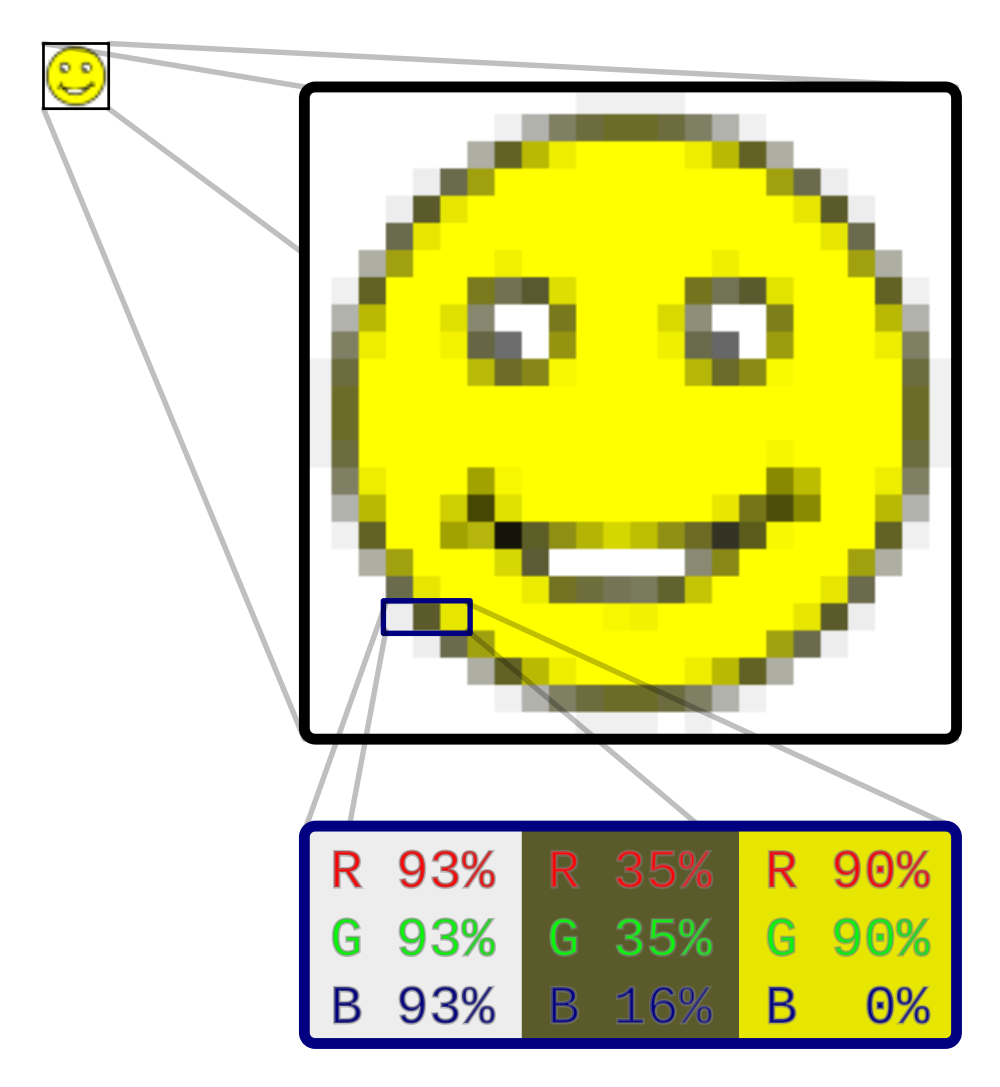
\includegraphics[width=0.6\textwidth]{src/images/rgb-raster-image.png}
  \caption[Example of an RGB raster image]{Example of a RGB raster image\protect\footnotemark}
  \label{fig:rgb-raster-image}
\end{figure}
\footnotetext{Source (accessed 02/2016): \url{https://en.wikipedia.org}.}

%explicit
\newpage

\subsection*{Human visual perception}

In his manuscript 'Astronomia Pars Optica' from 1604, Kepler explains the use of both eyes for depth perception.
He defined the term binocular as the composition of two latin words, 'bini' for double and 'oculus' for eye.
With uniocular as 'uni' for one the sight with only one eye is meant.
Binocular vision is then the vision creatures having two eyes obtain while using them together according to Kepler.
According to \citeauthor{fahle1987wozu} \citep{fahle1987wozu} and \citeauthor{henson2000visual} \citep{henson2000visual} creatures with binocular vision have several advantages over creatures with only uniocular vision.
Not to mention all but three, the most important ones which affect the depth perception:

\begin{enumerate}
  \item Considering human beings, the second eye increases the field of view \citep{henson2000visual}. About 120 degrees are the binocular field of view (projected on both eyes) and two uniocular fields of view with about 40 degrees.
  \item This also leads to another advantage with occluded, half-occluded or non-occluded objects \citep{fahle1987wozu}. Looking at Figure \ref{fig:horopter}, the point $P$ is in focus of the human being. Something directly behind this point may be fully occluded by the object in point $P$. Most of the things besides are non-occluded. Something behind this point $P$ may be half-occluded if it can be seen by either the left or the right eye.
  \item An advantage of having two eyes is the third-dimension human beings perceive, which leads to the binocular disparity or retinal disparity. Both terms are used in the literature and both mean the same: extracting depth information out of two coherent retinal images (obtained by the human eyes) \citep{cyganek2011introduction, fahle1987wozu}.
\end{enumerate}

\noindent Figure \ref{fig:horopter} depicts the mapping of the three points $R$, $P$ and $Q$ on the retina of each eye.
The letter $F$ stands for \textit{foveae} in which the visual axis ends.
The eye is constructed out of photoreceptor cells, mainly rods and cones.
The rods are necessary for seeing at night while the cones are responsible for humans being able to see the world sharp.
In the foveae is the peak of cones and it contains very few rods.
This means that the human visual system works the way that the visual axis joins the point of fixation with the foveae.
This can be seen in Figure \ref{fig:horopter} as the lines between $F$ of each eye to the point of fixation $P$.
Both eyes should be brought into convergence that the point of interest is projected onto the foveae of each eye.
Everything on the horopter (the circle) is corresponding (e.g. $P$ and $Q$), all points other than being on the horopter are non-corresponding ($R$) in terms of retinal disparity.
\newline\newline\noindent In the later described disparity algorithms which act like a tool for computers to be able to see the shift of pixels from the left image to the right image, the human being does somehow the same.
Humans experience the depth which is sensed unconsciously by the eyes and calculated by the brain in real-time.
With two eyes basically two slightly different images are obtained.
The brain acts as the computer which puts both coherent images together and extends the two-dimensional space into a three-dimensional space and calculates the position of the objects in the z-axis.

\begin{figure}[h!]
  \centering
  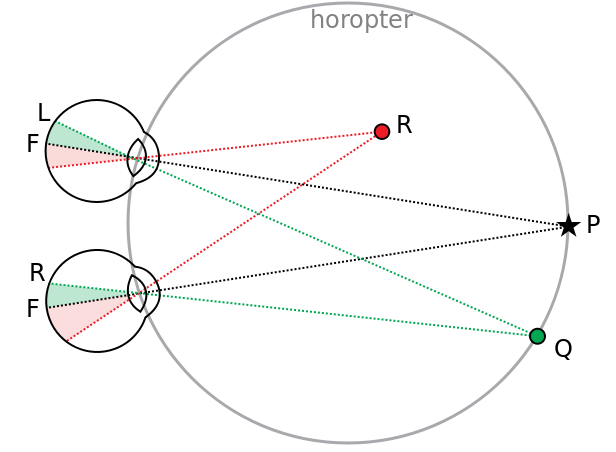
\includegraphics[width=0.6\textwidth]{src/images/horopter.png}
  \caption[Binocular vision with horopter principle]{Binocular vision with horopter principle\protect\footnotemark}
  \label{fig:horopter}
\end{figure}
\footnotetext{Source (accessed 02/2016): \url{https://en.wikipedia.org}.}

\noindent In contrast to the visual perception human beings perceive, computers need to do several steps to obtain disparity and calculate depth information:

\begin{itemize}
  \item identify objects,
  \item identify layers,
  \item match objects / pixels in both images,
  \item calculate the shift of the pixels from left to right, and
  \item obtain final depth values.
\end{itemize}

\noindent The human brain enables human beings to see and experience the real-world three-dimensional.
A computer has to be programmatically instructed to identify and group objects in both images \citep{block20133d, cyganek2011introduction}.
This is not an easy task as can be seen in the next sections.

\subsection*{Stereoscopy}

To paint the bigger picture, stereoscopy and the illusion of depth are introduced.
Stereoscopy is sometimes linked to the phrase 'the illusion of depth' as it is a technique used to add a third dimension to a flat image to simulate depth \citep{block20133d, lucas20133d}.
Specifically, the goal is to show each eye a slightly different image and thus achieve depth perception in our brain.
With so called stereoscope or special glasses depth perception can be transferred to the consumer in a cinema or at home via showing each eye a different image which then is composed to the final spatial perception.
\newline\newline\noindent There exist several techniques to create the stereoscopic effect. One of these glasses is the shutter system.
The concept of a shutter glass is that it cycles a block (meaning only one eye is dispatched to the screen) with a certain frequency (usually about 120 fps\footnote{frames per second}, resulting in 60 fps per eye) synchronously with the 3DTV.
This means that only one specific image is passed to exactly one of the consumers eyes.
So each eye is shown about 60 fps which naturally is experienced as flicker-free.
The older anaglyph 3D technique uses multiplied images tinted with red/cyan to filter out the respective image by the glasses filter foil, thus only one image is dispatched to one specific eye at a time.
Nowadays the anaglyph 3D technique is sometimes used in magazines to show 3D graphics.
As all techniques are not representing the real-world and the depth perception can be adjusted with for instance camera positioning (image one would reposition his eyes to perceive the real-world differently) they can be summarized as the illusion of depth.

\subsection*{Epipolar geometry}

The geometry of stereo images, called epipolar geometry, plays an important role in understanding the mathematical equations in the upcoming section.
The most important terms of epipolar geometry are:

\begin{itemize}
  \item image plane,
  \item baseline,
  \item epipole,
  \item epipolar line, and
  \item epipolar plane.
\end{itemize}

\noindent The \textit{image planes} in Figure \ref{fig:epipolar} and Figure \ref{fig:epipolar-rectified} are the blue surfaces which represent the captured image through the cameras $O_L$ and $O_R$.
The \textit{baseline} is the line joining both camera centers with the image plane. Focusing on the figures, the baseline is the line going from $O_L$ to $O_R$, as $O$ reflects the origin (camera center).
An \textit{epipole} is the joint of the baseline with the image plane, referring to the symbols $e_L$ and $e_R$.
The \textit{epipolar plane}, visualized as green triangle in Figures \ref{fig:epipolar} and \ref{fig:epipolar-rectified}, is determined by point $X$ and both origins $O_L$ and $O_R$.
It is the surface reflecting the z-axis, the depth.
An \textit{epipolar line} then is the intersection between the origin to the point of interest, in this particular case $X$, which lies on the epipolar plane and intersects the image plane.

\begin{figure}[h!]
  \centering
  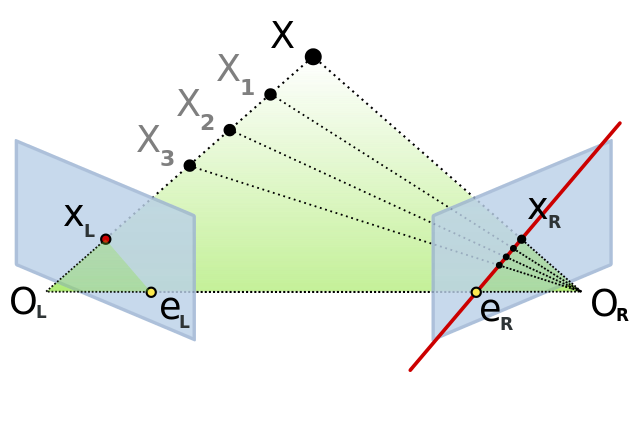
\includegraphics[width=0.7\textwidth]{src/images/epipolar.png}
  \caption[Epipolar geometry]{Epipolar geometry\protect\footnotemark}
  \label{fig:epipolar}
\end{figure}
\footnotetext{Source (accessed 02/2016): \url{https://en.wikipedia.org}.}

\noindent This results in an epipolar constraint \citep{cyganek2011introduction}:
Each image point $X_i$ of a space point in the image plane, e.g. consider point $X$ in Figure \ref{fig:epipolar} must lie on the corresponding epipolar line $\vec{O_LX}$.
More concrete focusing on Figure \ref{fig:epipolar}: this constraint states that the correspondence for a point on the epipolar line $\vec{O_LX}$ must lie on the line $\vec{e_rX_r}$.
As seen above Figure \ref{fig:epipolar} depicts the left and right view of an object in point $X$.
\newline\newline\noindent The Figures \ref{fig:epipolar} and \ref{fig:epipolar-rectified} both illustrate the epipolar geometry on a pair of unrectified images and the result after the rectification was done.
Rectification\footnote{Affine transformation (rotation and translation) neglecting geometric distortion to rectify the images.} is necessary to reduce the search-space from two-dimensional to one-dimensional.
For determining the exact position of $X$ (possible positions $X_i$ with $i = [1 \dots 3]$) the diagonal has to be scanned in the unrectified image.
In the rectified image only the horizontal needs to be investigated.
In the further proceeding this line is called the scanline which most of the algorithms operate on \citep{cyganek2011introduction, chowdhury2009new}.
After the rectification process the following two statements come true:

\begin{itemize}
  \item Epipolar lines are parallel to the x-axis (horizontal).
  \item Corresponding points are on the same y-axis (vertical).
\end{itemize}

\noindent Implicitly the following two assumptions were made:

\begin{itemize}
  \item the focal length $f$ of both cameras which captured the images are the same,
  \item the origin of one camera is the so called camera principal point (the joint of the optical axis with the image plane and the fovea counterpart) \citep{cyganek2011introduction}.
\end{itemize}

\noindent In conclusion, corresponding points are constrained to be on the same line and thus depth can be inferred by using triangulation and camera parameters.
Based on this, the investigations of stereo correspondence and the actual depth calculation using triangulation is discussed in more detail in the next sections.

\begin{figure}[h!]
  \centering
  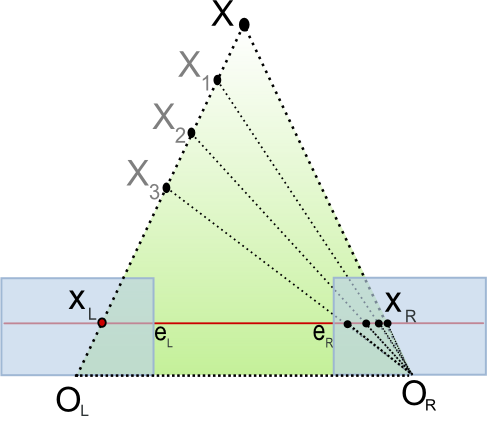
\includegraphics[width=0.6\textwidth]{src/images/epipolar-rectified.png}
  \caption[Epipolar geometry after image rectification]{Epipolar geometry after image rectification\protect\footnotemark}
  \label{fig:epipolar-rectified}
\end{figure}
\footnotetext{Source (accessed 02/2016): \url{https://en.wikipedia.org}.}

%explicit
\newpage

\section{Stereo correspondence}

Stereo correspondence can be seen as a pixel labelling problem \citep{wanner2013reconstructing, cyganek2011introduction} between two (or more) stereo images.
The essential problem is to find corresponding pixels in images of different cameras and needs to be solved.
Without knowing which points belong to each other in two separate stereo images, no conclusions can be drawn for instance calculating the disparity.
Henceforth, while talking about images for stereo matching, rectified images are implicitly meant.
If images are existing in an unrectified unaligned version then as a preprocessing step the images will be rectified.

\subsection*{Constraints}

Stereo matching algorithms rely on several assumptions about the real-world.
From the pioneer work of \citeauthor{marr1976cooperative} \citep{marr1976cooperative} the following constraints can be reasoned which are important for the development of such algorithms (also cf. \citep{cyganek2011introduction, wanner2013reconstructing,kack2004robust}):
\newline\newline\noindent \textit{As a short remark: $X_i$ is a point on a scanline in image $i$ ($i$ can be replaced with either $L$ for left or $R$ for right side) and thus only the x-position is mentioned.}

\begin{description}
  \item[Uniqueness] \hfill \\ As each pixel on a surface has one unique physical position in space, each pixel from each image has at most one disparity value.
  \item[Continuity] \hfill \\ The term smoothness constraint is also mentioned in the literature. Disparity can vary but smoothly almost everywhere in an image except at object boundaries which represent a discontinuity in depth, i.e. the difference of adjacent points should be small $||X_{L_1} - X_{R_1}| - |X_{L_2} - X_{R_2}|| < \varepsilon$.
  \item[Epipolar] \hfill \\ Recapture of the epipolar constraint from the section before: corresponding image points have to lie on the corresponding epipolar lines. If the epipolar lines are known to be parallel to the x-axis, the search space can be reduced to a 1D search space along the epipolar lines.
  \item[Ordering] \hfill \\ Following up the epipolar constraint: if the epipolar lines run in parallel to the x-axis, multiple consecutive image points have to lie on the same corresponding epipolar line in the same ordering.
  \item[Limit] \hfill \\ There is a defined disparity maximum (limit) $d_{max}$ holding $|X_L - X_R| < d_{max}$, defining the maximum disparity value which can be found in a stereo image. Hence, $d(x,y)$ is in the range $[0 \dots d_{max} - 1]$.
  \item[Lambertian] \hfill \\ Algorithms for stereo matching also rely on the assumption of opaque lambertian surfaces, meaning a surface that reflects light equally into all directions and thus appears equally bright independent from where light is coming and where the camera is placed. Thus the algorithms can expect the intensities and colors of corresponding points to be almost the same.
\end{description}

\noindent Besides those constraints there also exist some common pitfalls which can disturb the result of algorithm.

\subsection*{Common pitfalls}

Algorithms are using different metrics to analyze similarities in images along scanlines, in whole areas, or at a global view to then estimate the disparity.
This can be challenging especially considering the upcoming traps.
On the one hand, potential issues from the camera setup can be challenging, such as:

\begin{itemize}
  \item photometric distortions,
  \item noise,
  \item calibration error of the cameras.
\end{itemize}

\noindent On the other hand, the scenery can be tricky:

\begin{itemize}
  \item specularities and reflections,
  \item transparent objects,
  \item matching ambiguity,
  \item occlusions (missing data) and discontinuities.
\end{itemize}

\noindent These issues also challenge the algorithms to stereo match the pixels correctly.
With matching ambiguities, constant or low-contrast regions are meant.
A good example for that are textureless regions or repetitive structures.
Textureless regions could contain a small set of matching pairs of pixels, other pixels of that region could be erroneously assumed the same.
The presented constraints support the algorithms regarding those pitfalls.

\subsection*{Simplified stereo matching}

Figure \ref{fig:stereo-matching} depicts a simplified example of how stereo matching works on a one-dimensional search space:
there exist two arrays with $length = 5$, one in the left and one in the right image.
Assuming the top row $[p \dots t]$ reflects one row in the left image.
The bottom row $[u \dots y]$ accordingly the same row in the right image.
The pixel $p$, $q$, $w$ and $y$ are unmatched, e.g. occluded.
Having a function $d(z)$ which returns the disparity for a given element $z$ in those arrays, $d(r) = -2$ means the shift two to the left.
Accordingly $d(s) = -2$ and $d(t) = -1$.

\begin{figure}[h!]
  \centering
  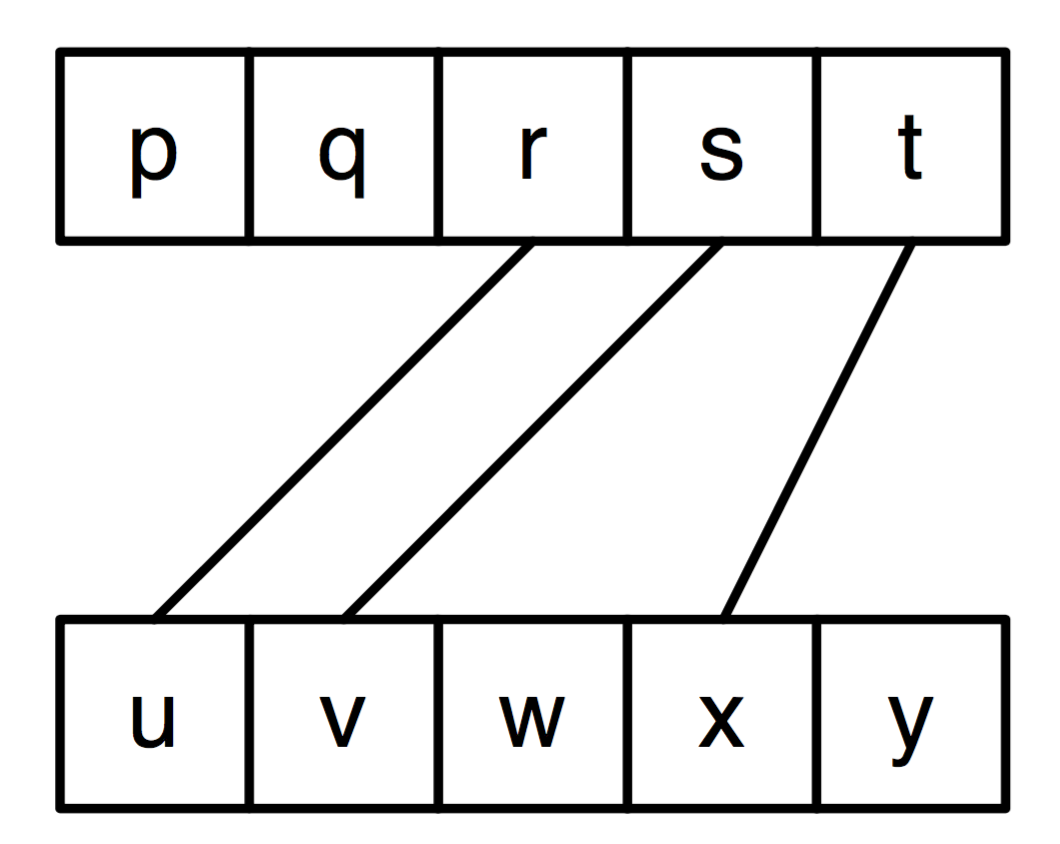
\includegraphics[width=0.3\textwidth]{src/images/stereo-matching.png}
  \caption[Two arrays illustrating stereo matching on a 1D search space]{Two arrays illustrating stereo matching on a 1D search space \citep{kack2004robust}.}
  \label{fig:stereo-matching}
\end{figure}

\noindent Up to this point the epipolar geometry and the challenge with stereo matching were introduced.
The upcoming section defines disparity, illustrates the disparity map, and the depth calculation.

\section{Disparity map between stereo images}

In the last two sections epipolar geometry and the problem with stereo correspondence were introduced.
In this section the focus is on the term disparity, how disparity can be visualized via disparity maps, and how the depth can be calculated out of those disparity values.

\subsection*{Disparity}

The disparity is the shift of a pixel / object (feature) between two or more images.
An object may appear at position $(x_1,y_1)$ in the left one and at position $(x_2,y_2)$ in the right one.
The disparity is the shift from the left position to the right one.
With $P_i$ declaring a point, left or right side, the following represents the disparity for two points in a two-dimensional space utilizing the pythagorean theorem:

\begin{equation}
  D(P_L,P_R) = \sqrt{D^2_X(P_L,P_R) + D^2_Y(P_L,P_R)}
\end{equation}

\noindent Henceforth, as the assumption of rectified images was made, only the horizontal disparity $D_X$ is meant by the term 'disparity'.

\begin{equation}
  D_X = |X_1 - X_2|
\end{equation}

\noindent In other words, having a pixel $(x_1,y_1)$ in a reference image (left) $l$ and a pixel $(x_2,y_2)$ in our matching image (right) $r$ the correspondence is given by:

\begin{equation}
  x_2 = x + |d(x_1,x_2)|\quad \textrm{with}\quad y_1 = y_2,
\end{equation}

\noindent where $d(x,y)$ is the function which delivers values out of the disparity space $(x,y,d)$ computed by the algorithms.
\newline\newline\noindent Resulting in matching pixels from one image to another, the disparity for each pixel-wise combination is calculated as seen in the previous subsection (simplified stereo matching) and presented here.
Such disparities can also be seen as the inversed distances to observed objects.
As a matter of fact, at the border of each image some pixels can not be calculated caused by the non-existing counterpart for matching.
Those pixels with no fellow are called 'occluded' pixels.
For example, in some cases pixels are hidden in one image by an object due to the blocking line of sight of this object.

\subsection*{Disparity map}

In order to actually analyze the output of algorithms ground-truth data is necessary.
An algorithm normally outputs a disparity map reflecting the disparity space $(x,y,d)$.
This disparity map can be seen as matrix having the size of the original image ($m \times n$) and containing values ranging from $0$ to $d_{max} - 1$ utilizing one color channel (grayscale).
The maximum disparity can be set via parameter for most of the algorithms and a feasible value which yields to sound results is $64$.
For better visual analysis the disparity maps are usually normalized to values ranging from $0 - 255$ \citep{martull2012realistic, cyganek2011introduction, scharstein2002taxonomy}.
Figure \ref{fig:tsukuba} c) shows the ground-truth data representing the disparity map.
The disparity map depicts grayscale intensities with lighter gray representing pixels / objects closer to the camera.
\newline\newline\noindent Tying in with the term ground-truth \citeauthor{martull2012realistic} created the first "highly realistic CG dataset that properly models real-world imperfections, while providing accurate ground truth." \citep{martull2012realistic}.
Without such datasets bad evaluation of stereo matching algorithms can be made as there would been no reference to evaluate against.
Figure \ref{fig:tsukuba} shows the previous dataset of the University of Tsukuba, the well-known \textit{Head and lamp scene}.

\begin{figure}[h!]
\centering
\begin{tabular}{ccc}
\subfloat[left input image]{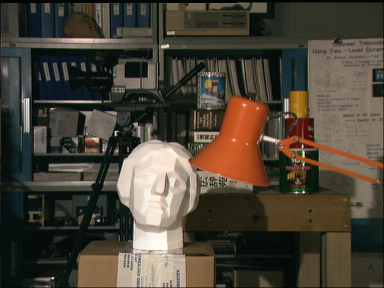
\includegraphics[width=0.3\textwidth]{src/images/tsukuba-imgL.png}} &
\subfloat[right input image]{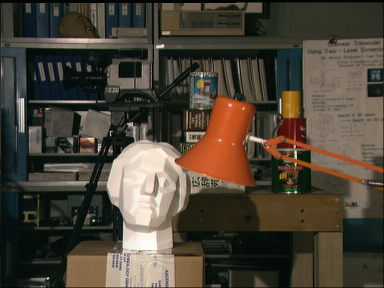
\includegraphics[width=0.3\textwidth]{src/images/tsukuba-imgR.png}} &
\subfloat[ground-truth data]{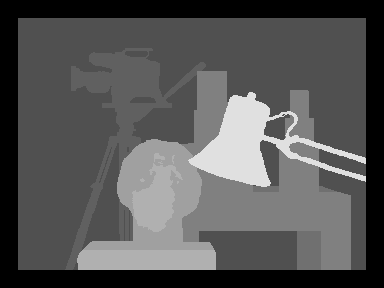
\includegraphics[width=0.3\textwidth]{src/images/tsukuba-dgt.png}}
\end{tabular}
\caption[Tsukuba benchmark stereo image pair of the University of Tsukuba]{Tsukuba benchmark stereo image pair of the University of Tsukuba \citep{martull2012realistic}.}
\label{fig:tsukuba}
\end{figure}

\noindent The input for a perfect algorithm would be the reference image (a) and the matching image (b).
After computation the result would be similar to the ground-truth data (c).
With evaluation metrics the computed disparity map is then compared to the ground-truth data.
Measuring instruments serve as a quality indicator for an algorithm's performance.
The above example is given for basic knowledge and understandability of how a disparity map actually looks like.
Details of this process are examined in the evaluation Chapter \ref{chap:eval}.

\subsection*{Depth calculation}

From an obtained disparity map and given camera parameters the depth can be calculated.
The mathematical description of the following equations has been introduced by \citeauthor{cyganek2011introduction} in Chapter 3.4.9 (Depth Resolution in Stereo Setups) of their book "\textit{An introduction to 3D computer vision techniques and algorithms}" \citep{cyganek2011introduction}.
Assuming the focal length of the camera's lens and the baseline\footnote{The distance between both image sources.} are known, the following holds:

\begin{equation}
  Z = \frac{f \cdot B}{d}\quad \textrm{and}\quad d = \frac{f \cdot B}{Z}
\end{equation}

\begin{equation}
  X = \frac{x \cdot Z}{f}\quad \textrm{and}\quad Y = \frac{y \cdot Z}{f}
\end{equation}

where:

\begin{itemize}
  \item $Z$ is the distance along the z-axis (camera axis),
  \item $f$ is the focal length,
  \item $B$ is the baseline (in meters),
  \item $d$ is the disparity of the point.
\end{itemize}

\noindent After $Z$ is determined, $X$ and $Y$ can be calculated using the usual projective camera equations (2.4-2.5) where the point $(x,y)$ is the pixel location in the 2D reference image and $(X,Y,Z)$ describes the real 3D position \citep{scharstein2002taxonomy, cyganek2011introduction, block20133d, martull2012realistic}.
Figure \ref{fig:depth-estimation} depicts the depth calculation from disparity with $X$ being the estimated point and $d = x - x'$.
\newline\newline\noindent The following subsection describes the more general steps of how disparity algorithms work, known as the taxonomy.

\begin{figure}[h!]
  \centering
  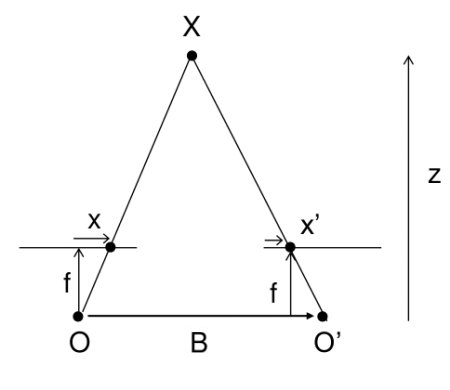
\includegraphics[width=0.6\textwidth]{src/images/depth-calculation.png}
  \caption[Depict of depth calculation from disparity.]{Depict of depth calculation from disparity.\protect\footnotemark}
  \label{fig:depth-estimation}
\end{figure}
\footnotetext{Source (accessed 02/2016): \url{http://docs.opencv.org}.}

%explicit
\newpage

\section{Disparity algorithms}

In the last sections different aspects affecting stereo matching were introduced.
To get a better understandability of the algorithm's technique, this section focuses on the diversity and taxonomy of disparity algorithms.

\subsection*{Diversity of disparity algorithms}

A lot of different algorithms exist and their workings differ slightly.
According to \citeauthor{cyganek2011introduction} \citep{cyganek2011introduction}, \citeauthor{scharstein2002taxonomy} \citep{scharstein2002taxonomy}, the following categories to separate disparity algorithms exist.
Some of these classifications are discussed in more detail the related work Chapter \ref{chap:related}.
\newline\newline\noindent First, the output of an algorithm is rated: they can create sparse or dense disparity maps.
On the one hand, most of the algorithms produce a dense disparity map meaning that almost every pixel got a corresponding shift value.
On the other hand, sparse algorithms only calculate values around, for instance, feature points (cf. feature matching).
One advantage of sparse algorithms compared to dense disparity algorithms is that they are normally faster in computation but limited in applications.
Approaches to interpolate sparse disparity maps into dense disparity maps exist, but they tend to produce inaccurate results in comparison to dense algorithms.
\newline\newline\noindent Second, \citeauthor{cyganek2011introduction} \citep{cyganek2011introduction} categorize direct and indirect methods.
Indirect methods are feature based or operate in the transformed image space (cf. Chapter 6.3.7 in \citep{cyganek2011introduction}).
Direct methods use intensity based measures.
\newline\newline\noindent Finally, disparity algorithms are classified into local and global methods:

\begin{itemize}
  \item Local Methods
  \begin{itemize}
    \item Feature matching
    \item Block (area) matching
  \end{itemize}
  \item Global Methods
  \begin{itemize}
    \item Belief propagation
    \item Graph cuts
    \item Dynamic programming
    \item Layering (hierarchical scale-space)
  \end{itemize}
\end{itemize}

\subsection*{Taxonomy of disparity algorithms}

\noindent Assumptions need to be made before starting to describe the taxonomy of disparity algorithms:

\begin{enumerate}
  \item The algorithm is fed with a pair of rectified images as input.
  \item The algorithm produces a dense integer disparity map, which means that disparity is estimated at each pixel.
  \item Most of the current algorithms works according to the following steps (see Figure \ref{fig:disparity-flow})
\end{enumerate}

\tikzstyle{rblock} = [text width=10em, rectangle, draw, fill=blue!18, text centered, rounded corners, minimum height=3em]
\tikzstyle{cloud} = [text width=6.5em, ellipse, draw, fill=blue!6, text centered, rounded corners, minimum height=3em]
\begin{figure}[h!]
  \centering
  \begin{tikzpicture}[node distance=4.8em, auto]
    \node [cloud] (input) {Pair of rectified images};
    \node [rblock, below of=input] (matchingcost) {Computing the matching cost};
    \node [cloud, below of=matchingcost] (DSI) {Disparity space image};
    
    \node [rblock, right of=computation, below of=DSI, node distance=6em] (aggregation) {Aggregation of the cost values};
    \node [rblock, left of=aggregation, below of=DSI, node distance=6em] (computation) {Computation of the disparity};    
    
    \node [cloud, below of=DSI, node distance=12em] (disparity) {Disparity map};
    \node [rblock, below of=disparity] (refinement) {Disparity refinement};

    \path [line] (input) -- (matchingcost);
    \path [line] (matchingcost) -- (DSI);
    \path [line] (DSI) -- node[anchor=north, xshift=-4.8em, yshift=1.0em] {for global methods}(computation);
    \path [line] (DSI) -- node[anchor=north, xshift=4.8em, yshift=1.0em] {for local methods}(aggregation);
    \path [line] (aggregation) -- (disparity);
    \path [line] (computation) -- (disparity);
    \path [line] (disparity) -- (refinement);
  \end{tikzpicture}
  \caption[Basic processing flow of typical disparity algorithms]{Basic processing flow of typical disparity algorithms, cf. \citep{cyganek2011introduction, scharstein2002taxonomy}.}
  \label{fig:disparity-flow}
\end{figure}

\noindent The upcoming subsections discuss the steps in more detail, especially regarding the computation of the matching cost and the subsequent aggregation.

%explicit
\newpage

\subsubsection{Matching cost functions}

At first, the similarities of pixels in both images are calculated.
In general, the literature shows matching cost as the dissimilarities of pixels.
The matching cost needs to be computed for the decision which pixel belongs to another.
Hence, the cost needs to be low for similar pixels.
Some of the matching criteria used for determining the matching cost are described in Table \ref{tab:overview-matching-cost-functions} cf. \citep{cyganek2011introduction, scharstein2002taxonomy, opencv_library, kanade1995development, hamzah2010sum}.

\begin{table}[h!]
\centering
\begin{tabular}{l|l}
  \hline
  \textbf{Method} & \textbf{Formula} \\ \hline \hline
  Sum of absolute differences & $\displaystyle \sum_{i,j \in U} \left| I_1(x_L+i,y_L+j) - I_2(x_R+i,y_R+j) \right|$ \\
  Sum of squared differences & $\displaystyle \sum_{i,j \in U} (I_1(x_L+i,y_L+j) - I_2(x_R+i,y_R+j))^2$ \\
  Normalized cross-correlation & $\displaystyle \frac{1}{n} \sum_{x,y}\frac{(I_1(x_L,y_L) - \overline{I_1})(I_2(x_R,y_R) - \overline{I_2})}{\sigma_{I_1} \sigma_{I_2}}$ \\
  \hline
\end{tabular}
\caption{Most common similarity measures}
\label{tab:overview-matching-cost-functions}
\end{table}

\noindent $I_k(x,y)$ stands for an intensity value of the image $k$ at the point with given coordinates $(x,y)$.
The set $U = U(i,j)$ describes close-by points located around the point $(i,j)$.
The sum of absolute differences (SAD) similarity measure is one of the simplest ones and describes the difference between pixel values.
The absolute intensity differences of both images $I_1$ and $I_2$ are summed up for all adjacent pixels in the neighborhood (described with $U$).
Zero stands for the equality of both regions.
In optimal images nearly every pixel in the left image should have a corresponding pixel in the right image, fulfilling the constraints from the section before, and thus the calculated SAD should sum up to zero.
The lower the result, the more similar the pixels and the cheaper the matching cost are.
\newline\newline\noindent In the sum of squared differences (SSD) similarity measure the pixel differences are squared and summed up.
This measurement needs a bit more computational power and is usually chosen to discriminate high differences.
It can yield to better results if outliers need to be excluded and the difference is not strong enough while using SAD.
\newline\newline\noindent There also exist the normalized cross-correlation (NCC).
Cross-correlation measures the correlation between two intensity values in a point $(x,y)$.
The normalized cross-correlation subtracts the mean $\overline{I}$ of the intensities and divides by the standard deviation $\sigma_{I}$ to normalize the intensity values. This may be necessary to balance brightness variations.
NCC is excluded in most scientific investigations regarding disparity algorithms as it behaves similar to SSD (cf. \citep{hirschmuller2007evaluation, scharstein2002taxonomy, cyganek2011introduction}).

%explicit
\newpage

\subsection*{Disparity space image}

Related to the disparity space introduced in the section before, the disparity space image (DSI) should be defined.
The DSI is an image or a function over a continuous or discretized version of the disparity space $(x,y,d)$ and represents the matching cost (i.e. the dissimilarity) of a given $d(x,y)$.
It can be imagined as a three-dimensional matrix with the x-axis meaning the column, the y-axis the disparity and each combination the matching cost for that particular value as the z-axis.
The disparity space image $C(x,y,d)$ is the result of the matching cost values over all pixels and all disparities, where the function $C$ that denotes the matching cost for the given input parameter.
This leads to the aggregation step, during which the matching cost form the final disparity for local methods.

\begin{figure}[h!]
  \centering
  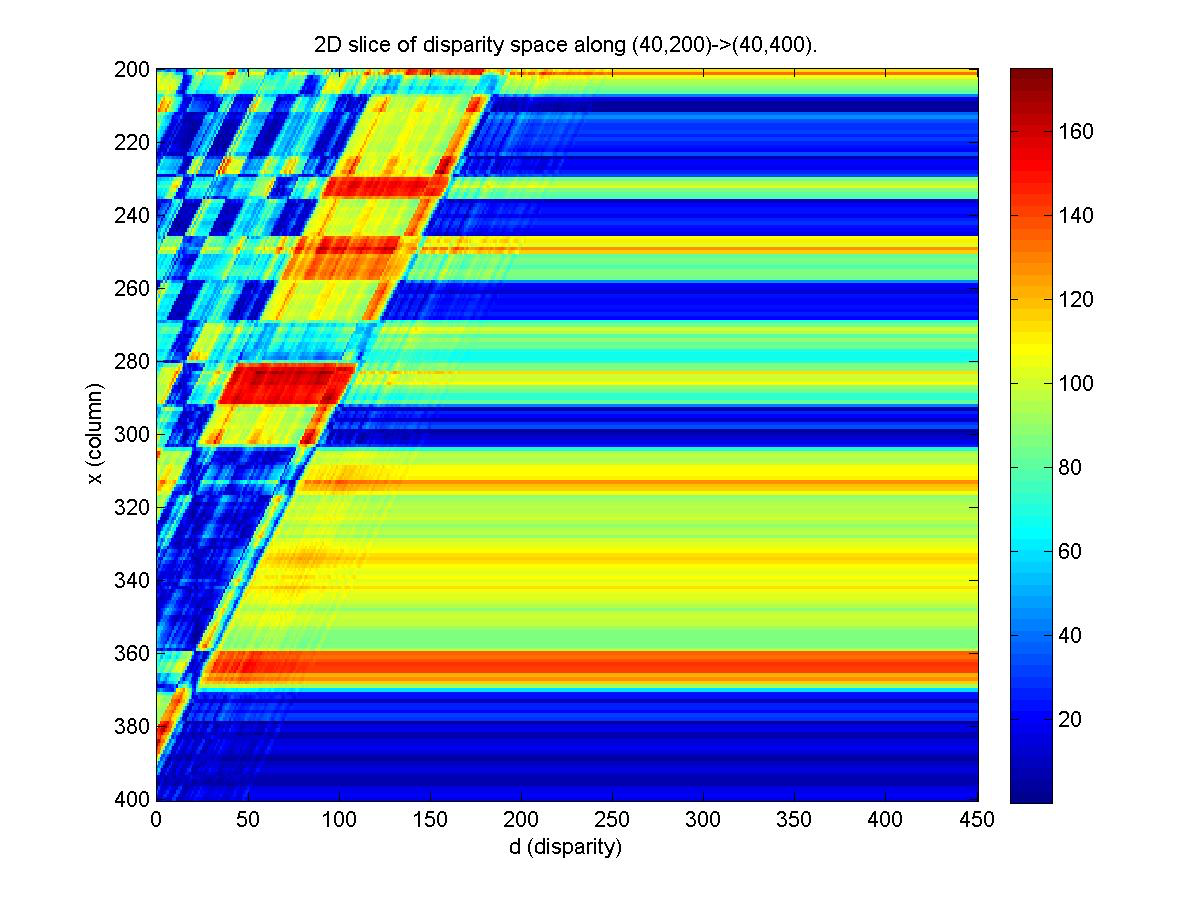
\includegraphics[width=1.0\textwidth]{src/images/dsi.png}
  \caption[Disparity space image]{Illustration of a disparity space image.\protect\footnotemark}
  \label{fig:dsi}
\end{figure}
\footnotetext{Source (accessed 03/2016): \url{http://www.cs.virginia.edu/~cab6fh/CV_4/WRITEUP.html}.}

\subsubsection{Aggregation}

In the aggregation step the decision has to be made, which discrete set of disparities represents the scene best \citep{scharstein2002taxonomy}.
As the matching cost values over all pixels and all disparities are stored in the DSI the minimum for each row is chosen as the best matching pixel and thus declared as the corresponding pixel.
In other words: for every pixel the disparity with the lowest cost is selected.
This strategy is known as the winner takes it all (WTA). \citep{cyganek2011introduction, scharstein2002taxonomy}.
As the pixel with the lowest cost is chosen, the following holds:

\begin{equation}
  d(x,y) = \arg\min_{d'} C(x,y,d').
\end{equation}

\subsubsection{Disparity computation}

After the aggregation, the actual disparity is computed in this step.
It is split up for the two different methods: local and global.
\newline\newline \noindent \textbf{(i) Local methods.} Local methods focus on the matching cost computation and the cost aggregation steps.
The final disparity computation is trivial as the minimum cost value (least dissimilarities) over each row is chosen (WTA).
\newline\newline\noindent \textbf{(ii) Global methods.} In contrast to local methods, global methods unify the three basic steps into a single one by defining an energy function to be minimized.
It ties in with the labelling problem \citep{tamassia2013handbook}.
A row in the DSI can be imagined as the different labels (i.e. disparity values) one pixel can receive.
The labelling problem describes the search of the disparity as the choice of the correct label.
Each pixel should only have one label assigned in the end.
\newline\newline\noindent Let $P$ be a set of pixels and $D$ a set of disparities. The energy function aims to find a disparity $d$ which minimizes some energy:

\begin{equation}
  E(d) = E_{data}(d) + \lambda E_{smooth}(d).
\end{equation}

\noindent The data term $E_{data}(d)$ defines the matching cost for a given disparity function $d$ and expresses how well the disparity function $d$ matches with the input image pair.
$C$ is the matching cost DSI:

\begin{equation}
  E_{data}(d) = \sum_{(x,y)} C(x,y,d(x,y)).
\end{equation}

\noindent As each pixel should be matched to a good find in the other image but simultaneously the adjacent pixels should be normally piecewise smooth, i.e. about the same value / intensity, the smoothness term $E_{smooth}(d)$ is introduced to reflect that (cf. stereo correspondence constraints).
The $\lambda$ is introduced to control how much the smoothness term should influence the overall data term.
To make the smoothness term computationally affordable it is, depending on the algorithm, usually restricted on the differences between adjacent pixel disparities \citep{scharstein2002taxonomy, cyganek2011introduction}, i.e. the disparity gradient:

\begin{equation}
  E_{smooth}(d) = \sum_{(x,y)} p(d(x,y) - d(x+1,y)) + p(d(x,y) - d(x,y+1)),
\end{equation}

\noindent where $p$ is a "monotonically increasing function of disparity difference" \citep{scharstein2002taxonomy}.
Depending on the used algorithm, other smoothness term functions exist.
The optimization problem to solve is defined as the minimization of the energy function, i.e.:

\begin{equation}
  D = \arg\min_{d} E(d),
\end{equation}

\noindent where $D$ is the disparity map containing the final values for every $(x,y)$ and $d$ a set of parameters or a disparity function affecting the energy value.
\newline\newline\noindent The search space for finding a solution is large, as an $n \times m$ image with $k$ disparities has about $k^{n \times m}$ possible solutions.
According to \citeauthor{scharstein2002taxonomy} \citep{scharstein2002taxonomy}, \citeauthor{cyganek2011introduction} \citep{cyganek2011introduction} finding the global minimum is \textit{NP-hard}.
The related work in Chapter \ref{chap:related} gives an introduction into solving those optimization problems.

\subsubsection{Disparity refinement}

Disparity refinement can be seen as an optional post-processing step some algorithms perform automatically or may be requested manually.
Refinement steps can also be implemented independently from the algorithm as they are executed on the final disparity maps.
Sometimes the literature mentions those as clean-up steps.
Here is a list of some known refinement steps:

\begin{itemize}
  \item Sub-pixel estimation for higher accuracy.
  \item Disparity verification with left-to-right and right-to-left disparity map comparison (can also detect occluded areas).
  \item Filtering of disparity values, for instance using a median filter to remove mismatches.
  \item Interpolation of missing values: can be necessary when using an algorithm which produces a sparse disparity map.
\end{itemize}

\subsubsection{Simplified block matching}

\noindent For demonstration purpose of a working local disparity algorithm, block matching, also known as area matching, is sketched in a simplified version.
The following algorithm assumes rectified images.
Thus, the algorithm is executed along the scanlines.

\begin{enumerate}
  \item Divide the images in blocks of the size $m \times n$ (e.g. $8 \times 8)$.
  \item Find the corresponding block along the scanlines as shown in Figure \ref{fig:tsukuba-block}, i.e. the block with the lowest matching cost (e.g. sum of absolute differences).
  \item Calculate for this block the displacement (the shift from left to right image) which results in the disparity.
  \item This yields in the final, ideally \textit{bijective}\footnote{Considering two sets, for each element of the first set a corresponding element of the second set is found. It also holds that both sets contain the same amount of elements. Thus, it is a one-to-one correspondence which also works inversely.} disparity map after finding the corresponding block from the left to the right image and vice versa. If a block could not be matched the bijective criteria is not fulfilled.
\end{enumerate}

\begin{figure}[h!]
  \centering
  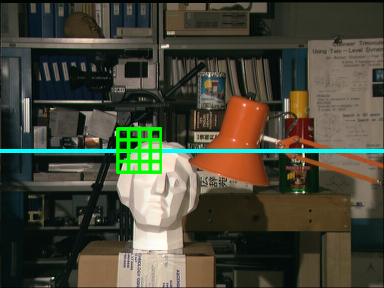
\includegraphics[width=0.5\textwidth]{src/images/tsukuba-block.png}
  \caption{Illustration of block matching along a scanline.}
  \label{fig:tsukuba-block}
\end{figure}

\noindent In general, block matching leads to more accurate results with smaller window sizes.
A bigger window leads to more smoothing which results in lower noise.
The window size depends on the image size and its content.
Therefore, no general assumption can be made.
For each scenery the window size should be adjusted individually.

\section{Sub-pixel accuracy}

As seen in the sections before, the disparity algorithms produce a disparity map consisting of integer values only.
For most of the imaginable applications integer values should be enough.
However, the world is continuous and there are applications which rely on accurate disparity estimations.
For instance, having no sub-pixel values, image-based rendering produces an image for visualizing the disparity map, which can appear to be made up of many thin shearing layers \citep{scharstein2002taxonomy}.
To get an accurate sub-pixel value, the most common technique is to use curve fitting by utilizing an \textit{n-th} polynomial-order function.
In this particular case \citep{scharstein2002taxonomy}, a second-order polynomial function, i.e. a parabola is used.
The curve is fitted around three or more values of the matching measure.
The point of interest lies in the center of the chosen window (as Figure \ref{fig:sub-pixel-estimation} depicts).
The minimum of this parabola is the searched value \citep{cyganek2011introduction, scharstein2014high}.
\newline\newline\noindent Curve fitting with a second-order-polynomial in Figure \ref{fig:sub-pixel-estimation} works with three data points: $(d_{i-1}, m_{i-1})$, $(d_{i}, m_{i})$ and $(d_{i+1}, m_{i+1})$.
$d_i$ is the found integer value for disparity and $m_i$ is a match value for the displacement $d_i$.
With the curve fit a new minimum value $d_x$ is found which no longer needs to lie on the integer grid.

\begin{figure}[h!]
  \centering
  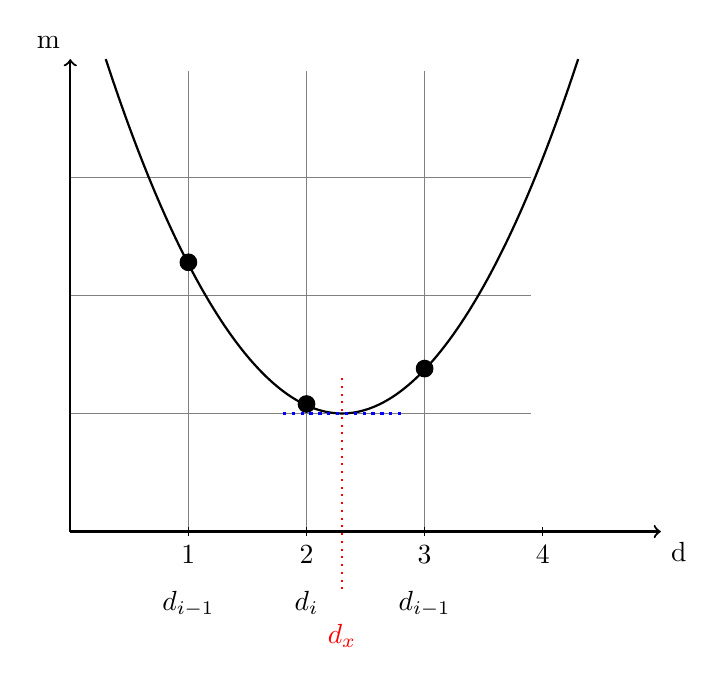
\begin{tikzpicture}[scale=1.5]
    %grid
    \draw[step=1cm,gray,very thin] (0,0) grid (3.9,3.9);
    %axes
    \draw[thick,->] (0,0) -- (5,0) node[anchor=north west] {d};
    \draw[thick,->] (0,0) -- (0,4) node[anchor=south east] {m};
    \foreach \x in {1,2,3,4}
      \draw (\x cm,1pt) -- (\x cm,-1pt) node[anchor=north] {$\x$};
    \draw (1cm,-12pt) node[anchor=north] {$d_{i-1}$};
    \draw (2cm,-12pt) node[anchor=north] {$d_{i}$};
    \draw (3cm,-12pt) node[anchor=north] {$d_{i-1}$};
    
    \draw[red] (2.3cm,-20pt) node[anchor=north] {$d_x$};
    %parabola
    \draw[thick] (2.3,1) parabola (0.3,4);
    \draw[thick] (2.3,1) parabola (4.3,4);
    %points
    \draw (1,2.28) circle[radius=2pt];
    \fill (1,2.28) circle[radius=2pt];
    \draw (2,1.08) circle[radius=2pt];
    \fill (2,1.08) circle[radius=2pt];
    \draw (3,1.38) circle[radius=2pt];
    \fill (3,1.38) circle[radius=2pt];
    %lines
    \draw[dotted,blue,very thick] (1.8,1) -- (2.8,1);
    \draw[dotted,red,thick] (2.3,1.3) -- (2.3,-0.5);
  \end{tikzpicture}
  \caption{Sub pixel estimation of a disparity value around adjacent pixels.}
  \label{fig:sub-pixel-estimation}
\end{figure}

\section{Optical flow}

Similar to the problems discussed in the section before, optical flow is also an image matching problem.
The optical flow is defined as vectors describing small local displacements like moving objects or camera motion between two consecutive frames \citep{cyganek2011introduction, opencv_library}.
The principle of the matching problem of images is comparable to disparity algorithms.
The main difference is that instead of analyzing left and right image, a scene is investigated and the disparity describes small local vectors.
To be more precise, the optical flow relies on the assumption that a certain point $(x_1, y_1)$ in a frame at time $t_1$ will be matched to a point $(x_2, y_2)$ in a frame at time $t_2$.
Different approaches for estimating the optical flow of pixels exist, like:

\begin{itemize}
  \item Correlation or block-matching,
  \item feature tracking,
  \item energy-based methods, or
  \item gradient-based methods.
\end{itemize}

\noindent Optical flow is heavily used in autonomous driving, automated traffic surveillance systems and video compression like H.264 \citep{cohen1999detecting, richardson2004h, kondermann2015stereo, menze2015object}.
Recently a dataset containing ground-truth data of real-world sceneries regarding optical-flow information was released by \citeauthor{kondermann2015stereo}.
Figure \ref{fig:optical-flow-estimation} shows an example of estimating the movement of a vehicle.
In the left image of Figure \ref{fig:optical-flow-estimation} most of the vectors are null as no local displacement can be estimated.
Only a few vectors (small white dots) near the vehicle illustrate the displacements.

\begin{figure}[h!]
  \centering
  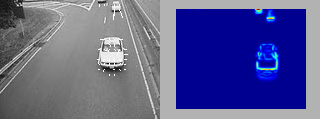
\includegraphics[width=1.0\textwidth]{src/images/optical-flow-estimation.jpg}
  \caption[Optical flow estimation]{Optical flow estimation to obtain motion vectors (left) and pixel velocity magnitudes (right).\protect\footnotemark}
  \label{fig:optical-flow-estimation}
\end{figure}
\footnotetext{Source (accessed 02/2016): \url{http://de.mathworks.com/discovery/optical-flow.html}.}
